\documentclass[../main.tex]{subfiles}

\begin{document}

\chapter{Introduction}
\label{cha:introduction}


\section{Plasmodesmata and their role in pathogen defence}
\label{sec:plasmodesmata}

\begin{figure}[ht]
  \centering
  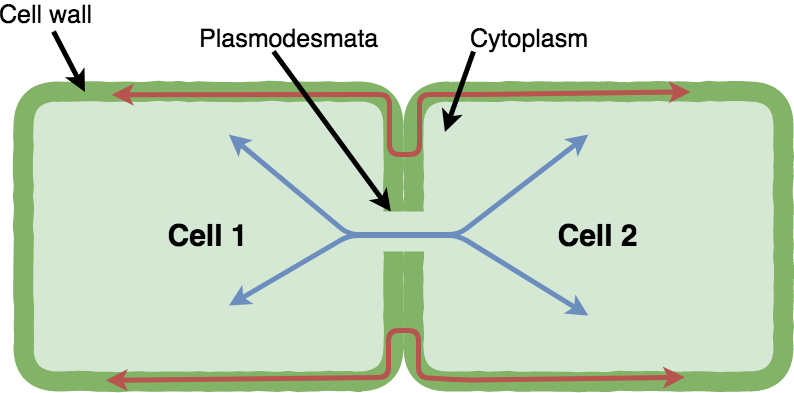
\includegraphics[width=0.5\columnwidth]{./figures/sympast+apoplast.png}
  \caption{\label{fig:pathways} Pathways for transfer between cells}
\end{figure}


\begin{figure}[!ht]
     \subfloat[First sub-figure\label{subfig-1:dummy}]{%
       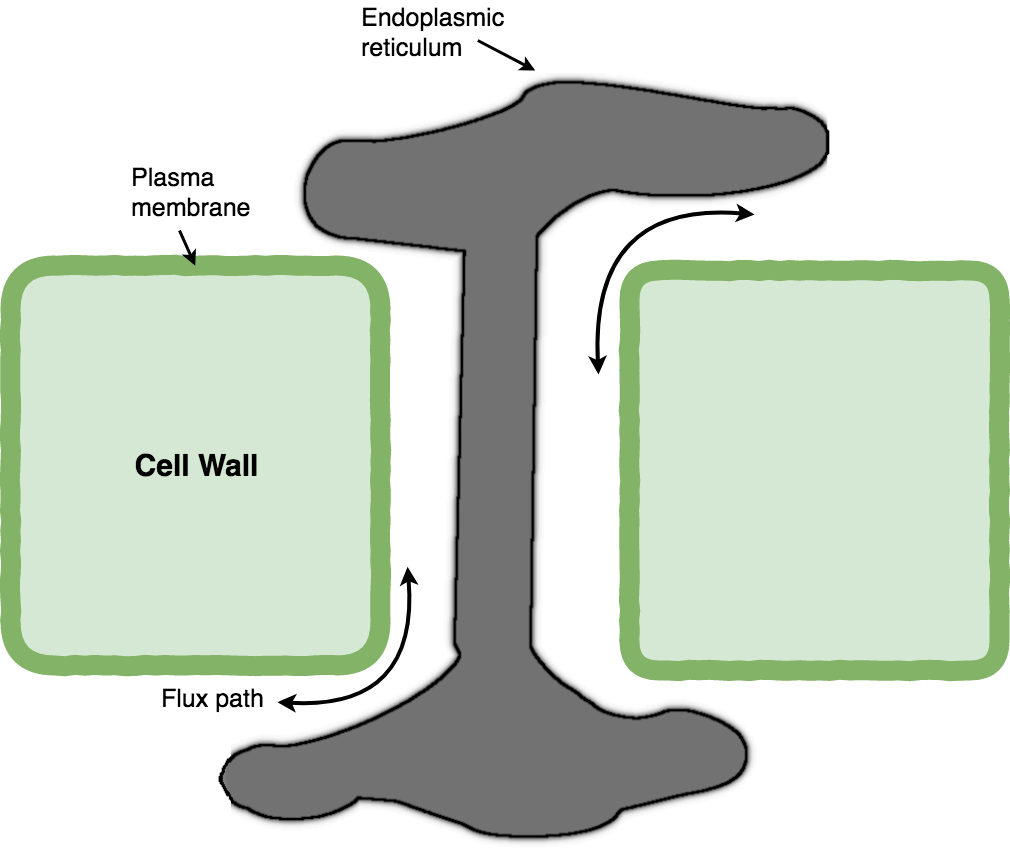
\includegraphics[width=0.4\columnwidth]{./figures/desmotubule.png}
     }
     \hfill
     \subfloat[First sub-figure\label{subfig-2:dummy}]{%
       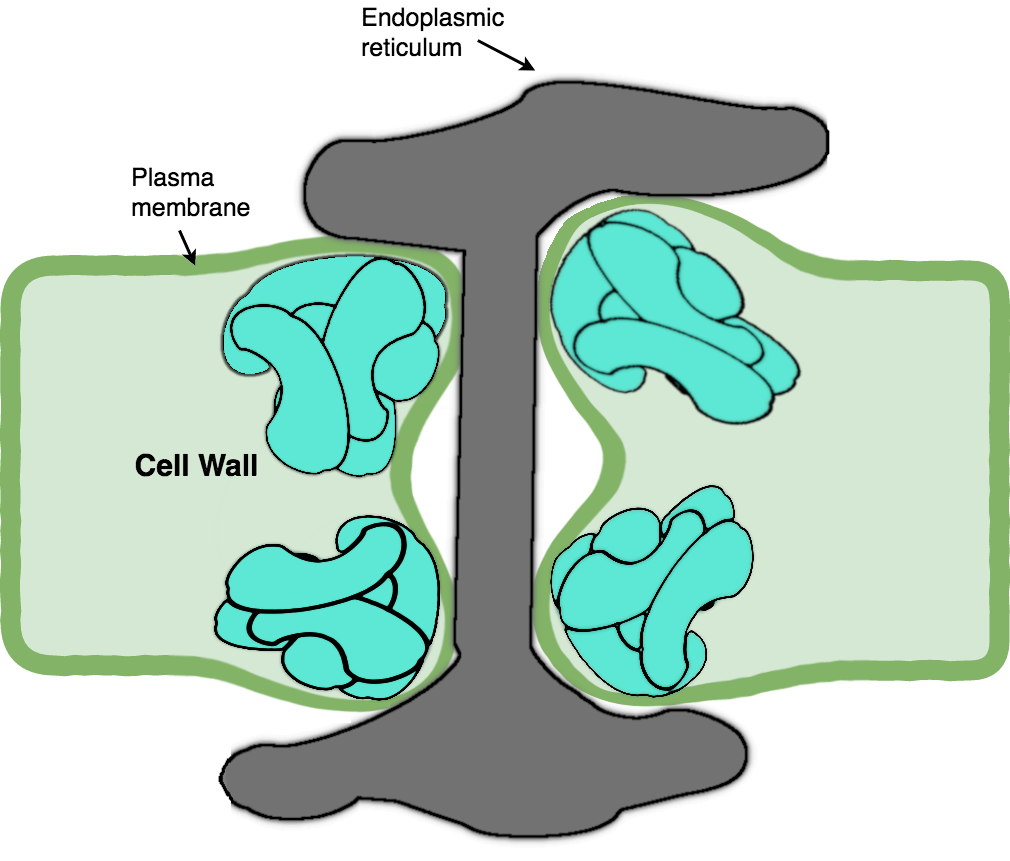
\includegraphics[width=0.4\columnwidth]{./figures/callose.png}
     }
     \caption{Dummy figure}
     \label{fig:dummy}
   \end{figure}


\section{Models concerning intercellular communication}
\label{sec:stateofmodelling}

\cite{deinumSimpleModelsComplex2013, deinumPlasmodesmaGeometryEffective2019}

\begin{figure}[ht]
  \centering
  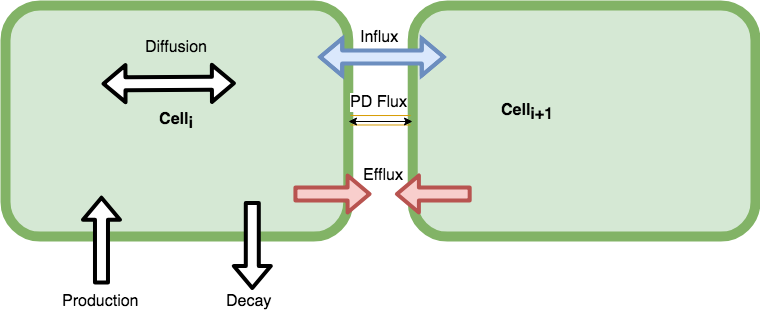
\includegraphics[width=\columnwidth]{figures/symplastic_model.png}
  \caption{\label{fig:deinummodel} Illustrated model of Dienum's work}
\end{figure}

   
\end{document}

%%% Local Variables:
%%% mode: latex
%%% TeX-master: "../main"
%%% End:
